% \documentclass[12pt,a4paper]{article}
\documentclass[12pt,a4paper,twoside]{article}

% --- Packages ---
\usepackage[utf8]{inputenc}
\usepackage[vietnamese]{babel}
\usepackage{graphicx}
\usepackage{booktabs}
\usepackage{amsmath, amssymb}
\usepackage{mathptmx} % Sets font to Times New Roman
\usepackage{hyperref}
\usepackage{geometry}
\usepackage{float}
\usepackage{caption}
\usepackage{enumitem}
\usepackage{listings}
\usepackage{xcolor}
\usepackage{fancybox}
\usepackage{longtable}
\usepackage{array}
\usepackage{indentfirst}


% \geometry{margin=2.5cm}
\geometry{inner=3.5cm, outer=2.0cm, top=2.5cm, bottom=2.5cm}
\setlength{\parindent}{1.0cm}


\hypersetup{colorlinks=true, linkcolor=blue, citecolor=blue, urlcolor=blue}

\begin{document}

\begin{titlepage}
\thispagestyle{empty}
\thisfancypage{\setlength{\fboxsep}{12pt}\fbox}{}

\begin{center}
{\textbf{\large{HỌC VIỆN CÔNG NGHỆ BƯU CHÍNH VIỄN THÔNG}}}\\
{\textbf{\large{KHOA CÔNG NGHỆ THÔNG TIN 1}}}\\
{\textbf{\large{\underline{\hspace{3cm}} o0o \underline{\hspace{3cm}}}}}\\

\vspace{1cm}

\includegraphics[width=0.4\linewidth]{figures/ptit_logo_1.png}

\vspace{1cm}
{\textbf{\huge{BÁO CÁO BÀI TẬP LỚN}}}\\
{\textbf{\huge{MÔN TRUY XUẤT THÔNG TIN}}}\\[0.8cm]
{\textbf{\Large{Đề tài: Khảo sát hệ thống truy xuất thông tin trên tập dữ liệu Cranfield sử dụng TF-IDF, BM25, QLM}}}\\[1cm]

\vspace{1.5cm}
\begin{tabular}{ll}
{\textbf{\large{Giảng viên hướng dẫn:}}} & {\textbf{\large{Phạm Đức Cường}}} \\
{\textbf{\large{Nhóm lớp:}}}  & {\textbf{\large{02}}}\\
{\textbf{\large{Nhóm bài tập lớn:}}}  & {\textbf{\large{09}}}\\
{\textbf{\large{Sinh viên thực hiện:}}} & {\textbf{\large{Ngô Việt Anh - B22DCKH004}}} \\
& {\textbf{\large{Nguyễn Đình Tiến - B22DCKH108}}}
\end{tabular}

\vspace{2cm}
{\textbf{\large{HÀ NỘI, 05/2026}}}

\end{center}
\end{titlepage}

\newpage
\thispagestyle{empty}
\mbox{}
\newpage

\tableofcontents
\newpage

% ===========================================================================
\section{Giới thiệu}
% ===========================================================================

Bài báo cáo trình bày quá trình xây dựng một hệ thống tìm kiếm thông tin (Information Retrieval -- IR) trên bộ dữ liệu Cranfield. Hệ thống bao gồm phần lõi thuật toán được lập trình bằng Python thuần và giao diện người dùng bằng Streamlit. Bốn mô hình xếp hạng được cài đặt và đánh giá: TF-IDF, Okapi BM25, Query Likelihood Model với Jelinek-Mercer Smoothing (QLM-JM) và Query Likelihood Model với Dirichlet Prior Smoothing (QLM-Dirichlet). Ngoài ra, hệ thống tích hợp module sửa lỗi chính tả dựa trên K-gram index và khoảng cách chỉnh sửa Levenshtein.

Bộ dữ liệu Cranfield gồm 1400 tài liệu khoa học về hàng không, 225 truy vấn, và bộ đánh giá liên quan (qrels) cho phép đánh giá hiệu suất tìm kiếm một cách khách quan. Đây là bộ dữ liệu kinh điển trong lĩnh vực IR, được sử dụng rộng rãi trong nghiên cứu và giảng dạy.

% ===========================================================================
\section{Cơ sở lý thuyết}
% ===========================================================================

% ---------------------------------------------------------------------------
\subsection{Chỉ mục ngược (Inverted Index)}
% ---------------------------------------------------------------------------

Chỉ mục ngược là cấu trúc dữ liệu nền tảng của hệ thống IR. Với mỗi term $t$ trong từ vựng, chỉ mục lưu trữ danh sách các tài liệu chứa $t$ cùng vị trí xuất hiện. Cấu trúc này cho phép truy vấn nhanh chóng thay vì phải duyệt tuần tự qua toàn bộ kho tài liệu.

Trong hệ thống này, chỉ mục ngược có dạng:
\[
\text{index}[t] = \{d_1: [p_1, p_2, \ldots], \; d_2: [p_1, \ldots], \; \ldots\}
\]
trong đó $d_i$ là mã tài liệu và $p_j$ là vị trí xuất hiện của term $t$ trong tài liệu đó.

% ---------------------------------------------------------------------------
\subsection{TF-IDF}
% ---------------------------------------------------------------------------

Mô hình TF-IDF kết hợp hai yếu tố: tần suất xuất hiện của term trong tài liệu (Term Frequency) và mức độ hiếm của term trong toàn bộ kho (Inverse Document Frequency). Trọng số của term $t$ trong tài liệu $d$ được tính như sau:

\begin{equation}
w_{t,d} = \text{tf}_{t,d} \times \text{idf}_t
\end{equation}

trong đó:
\begin{equation}
\text{tf}_{t,d} = 1 + \log_{10}(f_{t,d}), \quad f_{t,d} > 0
\end{equation}
\begin{equation}
\text{idf}_t = \log_{10}\left(\frac{N}{\text{df}_t}\right)
\end{equation}

$f_{t,d}$ là số lần xuất hiện của $t$ trong $d$, $N$ là tổng số tài liệu, và $\text{df}_t$ là số tài liệu chứa $t$. Điểm số cuối cùng được chuẩn hóa bằng căn bậc hai của độ dài tài liệu để tránh thiên lệch cho tài liệu dài.

% ---------------------------------------------------------------------------
\subsection{Okapi BM25}
% ---------------------------------------------------------------------------

BM25 là mô hình xếp hạng xác suất được phát triển dựa trên mô hình xác suất nhị phân độc lập (Binary Independence Model). So với TF-IDF, BM25 giới thiệu cơ chế bão hòa cho term frequency và chuẩn hóa độ dài tài liệu một cách rõ ràng qua hai tham số $k_1$ và $b$.

Điểm số BM25 được tính:
\begin{equation}
\text{score}(D, Q) = \sum_{t \in Q} \text{IDF}(t) \cdot \frac{f_{t,D} \cdot (k_1 + 1)}{f_{t,D} + k_1 \cdot \left(1 - b + b \cdot \frac{|D|}{\text{avgdl}}\right)}
\end{equation}

trong đó:
\begin{equation}
\text{IDF}(t) = \ln\left(\frac{N - \text{df}_t + 0.5}{\text{df}_t + 0.5} + 1\right)
\end{equation}

Tham số $k_1$ kiểm soát mức độ bão hòa của term frequency: giá trị $k_1$ lớn cho phép term frequency tiếp tục tăng ảnh hưởng, trong khi giá trị nhỏ hạn chế ảnh hưởng sau vài lần xuất hiện. Tham số $b$ kiểm soát mức chuẩn hóa độ dài: $b = 0$ bỏ qua chuẩn hóa, $b = 1$ chuẩn hóa hoàn toàn theo tỉ lệ độ dài so với trung bình.

% ---------------------------------------------------------------------------
\subsection{Query Likelihood Model --- Jelinek-Mercer Smoothing}
% ---------------------------------------------------------------------------

Mô hình Query Likelihood (QLM) tiếp cận bài toán xếp hạng từ góc độ mô hình ngôn ngữ. Ý tưởng chính là ước lượng xác suất sinh ra truy vấn $Q$ từ mô hình ngôn ngữ của tài liệu $D$, sau đó xếp hạng các tài liệu theo xác suất này.

Với phương pháp làm trơn Jelinek-Mercer, xác suất được tính bằng phép nội suy tuyến tính giữa mô hình tài liệu và mô hình tập dữ liệu:
\begin{equation}
P(t|D) = \lambda \cdot \frac{f_{t,D}}{|D|} + (1 - \lambda) \cdot P(t|C)
\end{equation}

trong đó $P(t|C)$ là xác suất của term $t$ trong toàn bộ tập dữ liệu (collection), và $\lambda \in (0, 1)$ là tham số làm trơn. Điểm số của tài liệu:
\begin{equation}
\text{score}(D, Q) = \sum_{t \in Q} \log P(t|D)
\end{equation}

Tham số $\lambda$ cân bằng giữa bằng chứng từ tài liệu cụ thể và bằng chứng từ toàn bộ tập dữ liệu. Giá trị $\lambda$ cao (gần 1) tin tưởng tài liệu nhiều hơn, phù hợp với truy vấn dài; giá trị thấp dựa nhiều vào thống kê toàn cục, phù hợp với truy vấn ngắn.

% ---------------------------------------------------------------------------
\subsection{Query Likelihood Model --- Dirichlet Prior Smoothing}
% ---------------------------------------------------------------------------

Phương pháp Dirichlet Prior coi mô hình tập dữ liệu như tiên nghiệm (prior) Dirichlet và cập nhật bằng bằng chứng từ tài liệu. Công thức:
\begin{equation}
P(t|D) = \frac{f_{t,D} + \mu \cdot P(t|C)}{|D| + \mu}
\end{equation}

Tham số $\mu > 0$ đóng vai trò trọng số của tiên nghiệm. Khi $\mu$ lớn, mô hình dựa nhiều vào thống kê toàn cục, phù hợp cho tài liệu ngắn. Khi $\mu$ nhỏ, mô hình dựa chủ yếu vào nội dung tài liệu. Một đặc điểm của Dirichlet so với Jelinek-Mercer là mức độ làm trơn tự động giảm theo độ dài tài liệu, vì $|D|$ xuất hiện ở mẫu số.

% ---------------------------------------------------------------------------
\subsection{K-gram Index và Khoảng cách Levenshtein}
% ---------------------------------------------------------------------------

K-gram index hỗ trợ tìm kiếm chịu lỗi (tolerant retrieval). Mỗi term trong từ vựng được phân tách thành các chuỗi con có độ dài $k$ (mặc định $k = 2$, tức bigram), kèm ký tự đánh dấu \texttt{\$} ở đầu và cuối. Ví dụ, term ``flow'' sinh ra các bigram: \texttt{\$f}, \texttt{fl}, \texttt{lo}, \texttt{ow}, \texttt{w\$}.

Khi nhận một từ không có trong từ vựng, hệ thống:
\begin{enumerate}
    \item Sinh các k-gram của từ cần sửa.
    \item Tra K-gram index để tìm các term ứng viên có hệ số Jaccard đủ lớn.
    \item Tính khoảng cách Levenshtein giữa từ cần sửa và mỗi ứng viên.
    \item Chọn ứng viên có khoảng cách nhỏ nhất (tối đa 2).
\end{enumerate}

Khoảng cách Levenshtein đo số phép chỉnh sửa tối thiểu (chèn, xóa, thay thế) cần thiết để biến đổi một chuỗi thành chuỗi khác. Thuật toán được cài đặt bằng quy hoạch động với độ phức tạp $O(m \times n)$.

% ---------------------------------------------------------------------------
\subsection{Các metric đánh giá}
% ---------------------------------------------------------------------------

Năm metric được sử dụng để đánh giá hiệu suất:

\textbf{Precision at K (P@K):} tỉ lệ tài liệu liên quan trong top-K kết quả.
\begin{equation}
P@K = \frac{|\{\text{tài liệu liên quan trong top-}K\}|}{K}
\end{equation}

\textbf{Recall at K (R@K):} tỉ lệ tài liệu liên quan được tìm thấy so với tổng số tài liệu liên quan.
\begin{equation}
R@K = \frac{|\{\text{tài liệu liên quan trong top-}K\}|}{|\text{tất cả tài liệu liên quan}|}
\end{equation}

\textbf{F1-Score at K:} trung bình điều hòa của P@K và R@K.
\begin{equation}
F1@K = \frac{2 \cdot P@K \cdot R@K}{P@K + R@K}
\end{equation}

\textbf{Mean Average Precision (MAP):} trung bình của Average Precision trên tất cả truy vấn.
\begin{equation}
\text{MAP} = \frac{1}{|Q|} \sum_{q \in Q} \text{AP}(q), \quad \text{AP}(q) = \frac{1}{|\text{Rel}_q|} \sum_{k=1}^{n} P@k \cdot \text{rel}(k)
\end{equation}

\textbf{Mean Reciprocal Rank (MRR):} trung bình nghịch đảo hạng của tài liệu liên quan đầu tiên.
\begin{equation}
\text{MRR} = \frac{1}{|Q|} \sum_{q \in Q} \frac{1}{\text{rank}_q}
\end{equation}

% ===========================================================================
\section{Thiết kế hệ thống}
% ===========================================================================

% ---------------------------------------\subsection{Giao diện Streamlit}
% ---------------------------------------------------------------------------

Giao diện được chia thành hai phần: thanh bên (sidebar) chứa bảng điều khiển cho phép chọn mô hình, điều chỉnh tham số qua thanh trượt, và bật/tắt sửa lỗi chính tả; phần chính hiển thị ô tìm kiếm, gợi ý sửa lỗi, và danh sách kết quả dưới dạng thẻ. Giá trị mặc định của các thanh trượt được lấy từ kết quả tinh chỉnh siêu tham số.

% ---------------------------------------------------------------------------
\subsection{Quy trình hoạt động và luồng xử lý}
% ---------------------------------------------------------------------------

Quy trình hoạt động của hệ thống được chia làm hai giai đoạn chính là xử lý ngoại tuyến và xử lý trực tuyến. Ở giai đoạn ngoại tuyến, hệ thống bắt đầu bằng việc tải tự động bộ dữ liệu Cranfield từ thư viện dữ liệu. Tập tài liệu thô sau đó được đưa qua pipeline tiền xử lý để chuyển thành chữ thường, tách thành các từ đơn, loại bỏ từ dừng và tiến hành rút gọn gốc từ bằng thuật toán Porter. Kết quả tiền xử lý được dùng để xây dựng hai cấu trúc dữ liệu quan trọng là chỉ mục ngược nhằm phục vụ truy xuất nhanh và chỉ mục K-gram phục vụ cho việc sửa lỗi chính tả. Toàn bộ các chỉ mục này cùng danh sách tài liệu thô và truy vấn gốc được lưu trữ dưới dạng bộ nhớ đệm cache trên ổ đĩa để tăng tốc độ khởi động cho những lần chạy sau.

Ở giai đoạn xử lý trực tuyến khi người dùng tương tác với giao diện Streamlit, quy trình xử lý truy vấn chịu lỗi được kích hoạt. Khi người dùng nhập một câu truy vấn bất kỳ, hệ thống sẽ tiến hành chuẩn hóa và tách câu thành danh sách các từ. Đối với mỗi từ, hệ thống kiểm tra xem từ đó có tồn tại trong từ vựng của tập dữ liệu hay không. Nếu phát hiện từ không có trong từ điển, hệ thống sẽ tự động tách từ lỗi này thành các chuỗi con hai ký tự (bigrams) rồi tra cứu trong chỉ mục K-gram để lấy ra danh sách các từ ứng viên chia sẻ chung các chuỗi con này. Hệ thống tính toán hệ số tương đồng Jaccard để lọc bớt các ứng viên kém chất lượng, sau đó áp dụng thuật toán quy hoạch động tính khoảng cách sửa lỗi Levenshtein để tìm từ trong từ điển có khoảng cách biến đổi nhỏ nhất (trong ngưỡng cho phép tối đa là hai). Từ sai chính tả sẽ được thay thế bằng từ chính xác để tạo ra câu truy vấn đã hiệu chỉnh.

Câu truy vấn sau khi hiệu chỉnh được đưa vào bộ tiền xử lý tương tự như tài liệu để thu được các gốc từ chuẩn. Dựa trên các gốc từ này, hệ thống truy xuất các danh sách tài liệu tương ứng từ chỉ mục ngược. Các mô hình xếp hạng được lựa chọn (như TF-IDF, BM25 hoặc QLM) sẽ tính toán điểm số tương đồng giữa câu truy vấn và từng tài liệu dựa trên các tham số cấu hình do người dùng thiết lập trên giao diện hoặc các tham số tối ưu có sẵn. Cuối cùng, danh sách tài liệu được sắp xếp theo điểm số giảm dần và hiển thị trực quan lên giao diện dưới dạng các thẻ kết quả kèm theo thông tin về thời gian phản hồi.

Quy trình tinh chỉnh siêu tham số và đánh giá hệ thống được thực hiện tự động thông qua các tập lệnh kiểm thử. Hệ thống thực hiện Grid Search duyệt qua toàn bộ không gian tham số của từng mô hình, tiến hành truy xuất kết quả cho tất cả 225 truy vấn thử nghiệm và tính toán các độ đo hiệu suất tại ngưỡng cắt K bằng mười. Bộ tham số nào mang lại giá trị MAP cao nhất sẽ được lựa chọn làm cấu hình tối ưu và ghi lại vào tệp cấu hình để giao diện Streamlit tự động nạp làm giá trị mặc định cho người dùng.

% ===========================================================================
\section{Thực nghiệm và kết quả}
% ===========================================================================

% ---------------------------------------------------------------------------
\subsection{Đánh giá với tham số mặc định}
% ---------------------------------------------------------------------------

Bảng~\ref{tab:baseline} trình bày kết quả đánh giá bốn mô hình với tham số tối ưu (sau Grid Search) trên toàn bộ 225 truy vấn. Kết quả truy xuất top 100, metric được tính tại $K = 10$.

\begin{table}[H]
\centering
\begin{tabular}{lccccc}
\toprule
\textbf{Mô hình} & \textbf{P@10} & \textbf{R@10} & \textbf{F1@10} & \textbf{MAP} & \textbf{MRR} \\
\midrule
TF-IDF             & 0.3053 & 0.4487 & 0.3368 & 0.4097 & 0.8061 \\
BM25               & 0.3191 & 0.4573 & 0.3482 & 0.4330 & 0.8292 \\
QLM (JM)           & 0.2996 & 0.4405 & 0.3306 & 0.4061 & 0.8091 \\
QLM (Dirichlet)    & 0.2991 & 0.4359 & 0.3287 & 0.4064 & 0.8075 \\
\bottomrule
\end{tabular}
\caption{Kết quả đánh giá với tham số tối ưu ($K = 10$). BM25: $k_1 = 2.0, b = 0.75$; QLM-JM: $\lambda = 0.3$; QLM-Dirichlet: $\mu = 250$.}
\label{tab:baseline}
\end{table}

Kết quả thực nghiệm cho thấy mô hình BM25 đạt hiệu suất vượt trội so với các phương pháp khác, dẫn đầu ở mọi chỉ số đánh giá với điểm số MAP đạt 0.4330 và điểm số MRR đạt 0.8292. Điều này cho thấy mô hình BM25 có khả năng sắp xếp các tài liệu thực sự liên quan lên các vị trí đầu tiên của danh sách kết quả một cách chính xác. Hiệu suất cao của BM25 xuất phát từ việc tích hợp tốt cơ chế bão hòa tần suất xuất hiện của từ khóa cùng với việc chuẩn hóa độ dài tài liệu một cách linh hoạt thông qua tham số bão hòa và tham số chuẩn hóa độ dài. 

Mô hình TF-IDF đứng thứ hai với điểm số MAP đạt 0.4097 và MRR đạt 0.8061, bám sát các mô hình còn lại nhờ cơ chế chuẩn hóa độ dài bằng căn bậc hai độ dài tài liệu, giúp hạn chế thiên vị đối với các tài liệu dài. Hai biến thể của mô hình ngôn ngữ truy vấn là QLM Jelinek-Mercer và QLM Dirichlet cho hiệu suất gần như tương đương nhau với điểm số MAP dao động xung quanh mức 0.406. Hiệu suất của hai mô hình ngôn ngữ này thấp hơn so với BM25 một phần do đặc thù của bộ dữ liệu Cranfield chỉ bao gồm các đoạn tóm tắt ngắn của các bài báo khoa học. Do văn bản tài liệu ngắn nên không gian xác suất để xây dựng mô hình ngôn ngữ tài liệu bị hạn chế và dễ bị nhiễu, dẫn đến việc ước lượng xác suất sinh truy vấn chưa đạt được hiệu quả tối đa như mô hình xác suất BM25.

% ---------------------------------------------------------------------------
\subsection{Tinh chỉnh siêu tham số}
% ---------------------------------------------------------------------------

Siêu tham số của ba mô hình BM25, QLM Jelinek-Mercer và QLM Dirichlet được tinh chỉnh thông qua phương pháp Grid Search để tối ưu hóa chỉ số MAP trên toàn bộ 225 truy vấn của bộ dữ liệu. Kết quả tinh chỉnh cho thấy sự biến động hiệu suất rõ rệt khi thay đổi các giá trị tham số, đồng thời giúp xác định được cấu hình tối ưu cho từng thuật toán xếp hạng.

Biểu đồ nhiệt ở Hình~\ref{fig:bm25_heatmap} thể hiện sự thay đổi điểm số MAP của mô hình BM25 theo sự kết hợp của hai siêu tham số là b và k1. Quan sát biểu đồ cho thấy tham số chuẩn hóa độ dài tài liệu b đóng vai trò quyết định đến hiệu suất hệ thống. Khi giá trị b tiến dần về không (tức là loại bỏ hoàn toàn cơ chế chuẩn hóa độ dài tài liệu), điểm số MAP sụt giảm rất mạnh. Điều này là do các tài liệu dài có xu hướng chứa nhiều từ khóa hơn sẽ bị đánh giá cao hơn một cách bất công nếu không được chuẩn hóa. Vùng tối ưu trên biểu đồ nhiệt tập trung xung quanh giá trị b bằng 0.75 và giá trị k1 bằng 2.0. Tại điểm tối ưu này, hệ thống đạt điểm số MAP cao nhất là 0.4330.

\begin{figure}[H]
\centering
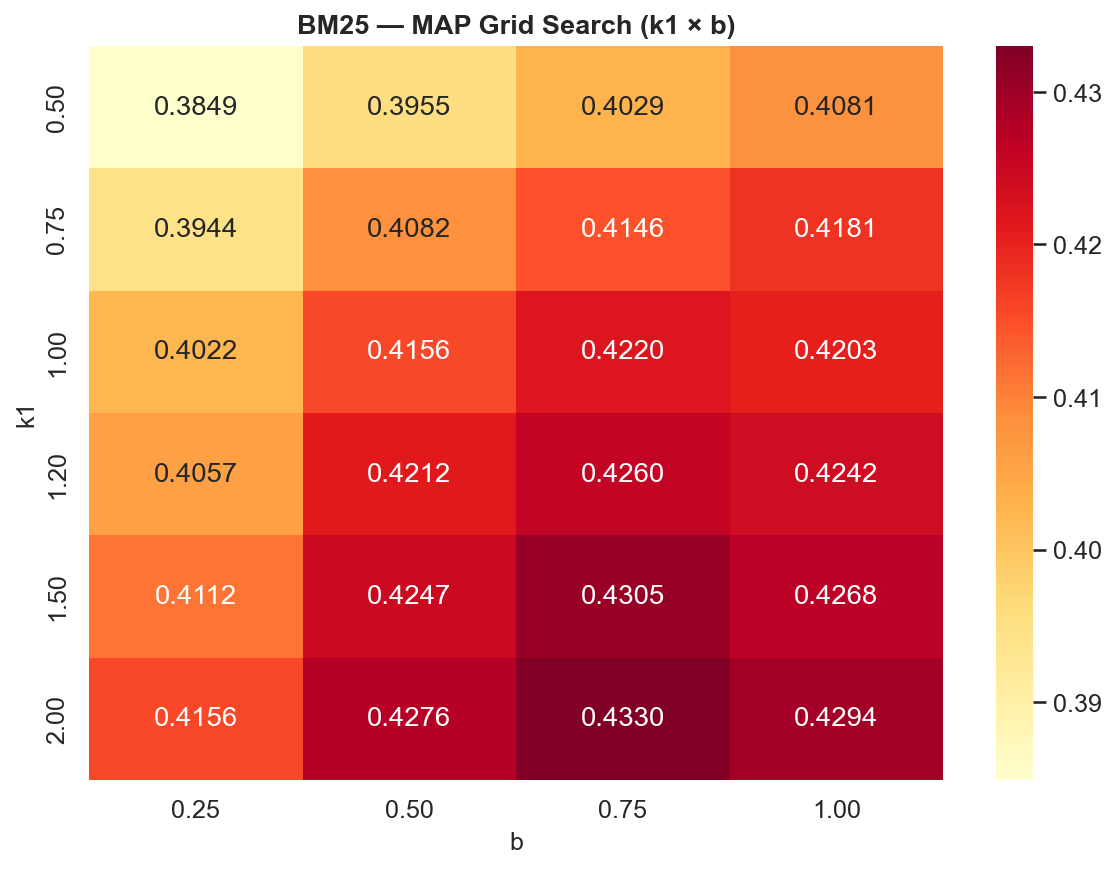
\includegraphics[width=0.6\textwidth]{figures/bm25_heatmap.png}
\caption{BM25 --- MAP theo Grid Search ($k_1 \times b$).}
\label{fig:bm25_heatmap}
\end{figure}

Đối với mô hình ngôn ngữ QLM sử dụng làm trơn Jelinek-Mercer, Hình~\ref{fig:qlm_jm} mô tả sự phụ thuộc của điểm số MAP vào tham số làm trơn lambda. Điểm số MAP đạt giá trị cực đại tại lambda bằng 0.3. Việc giá trị lambda tối ưu nằm ở mức thấp (0.3 thay vì sát mức 1.0) cho thấy mô hình cần dựa nhiều vào phân bố xác suất từ vựng trên toàn tập dữ liệu (collection model) để bổ sung và làm trơn cho mô hình ngôn ngữ của từng tài liệu đơn lẻ. Điều này hoàn toàn phù hợp với thực tế rằng các tài liệu ngắn trong tập dữ liệu Cranfield thường thiếu vắng nhiều từ khóa liên quan, do đó việc dựa vào tần suất từ vựng toàn cục giúp giảm thiểu hiện tượng gán xác suất bằng không cho các từ khóa truy vấn không xuất hiện trực tiếp trong tài liệu.

\begin{figure}[H]
\centering
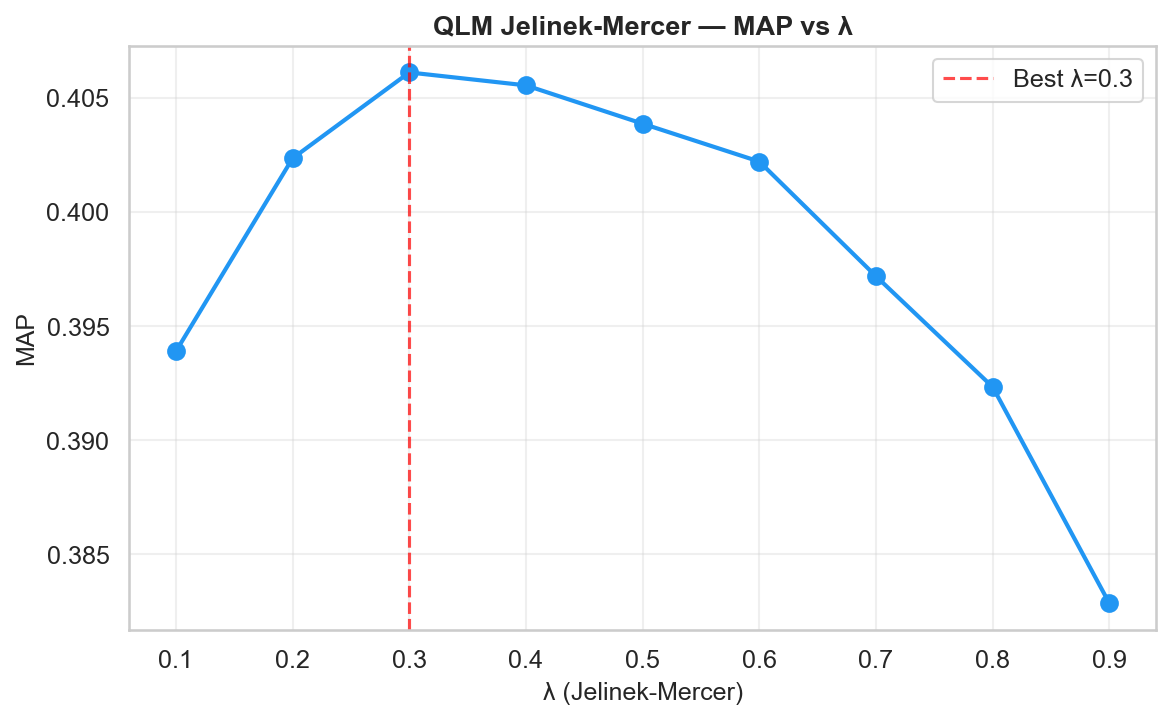
\includegraphics[width=0.6\textwidth]{figures/qlm_jm_lambda.png}
\caption{QLM Jelinek-Mercer --- MAP theo $\lambda$.}
\label{fig:qlm_jm}
\end{figure}

Đối với mô hình QLM sử dụng làm trơn Dirichlet Prior, Hình~\ref{fig:qlm_dir} thể hiện tác động của tham số giả định mu lên hiệu suất tìm kiếm. Điểm số MAP đạt đỉnh cao nhất tại mu bằng 250, sau đó giảm dần khi giá trị mu tiếp tục tăng lên các mức cao hơn. Giá trị mu tối ưu tương đối nhỏ (250) phản ánh trung bình độ dài tài liệu trong tập dữ liệu Cranfield khá ngắn, chỉ khoảng 103 từ đơn. Mức mu này cung cấp một lượng làm trơn vừa phải, giúp cân bằng tốt giữa thông tin thực tế có trong tài liệu ngắn và phân bố nền của toàn tập dữ liệu mà không làm lu mờ đi các đặc trưng riêng của tài liệu.

\begin{figure}[H]
\centering
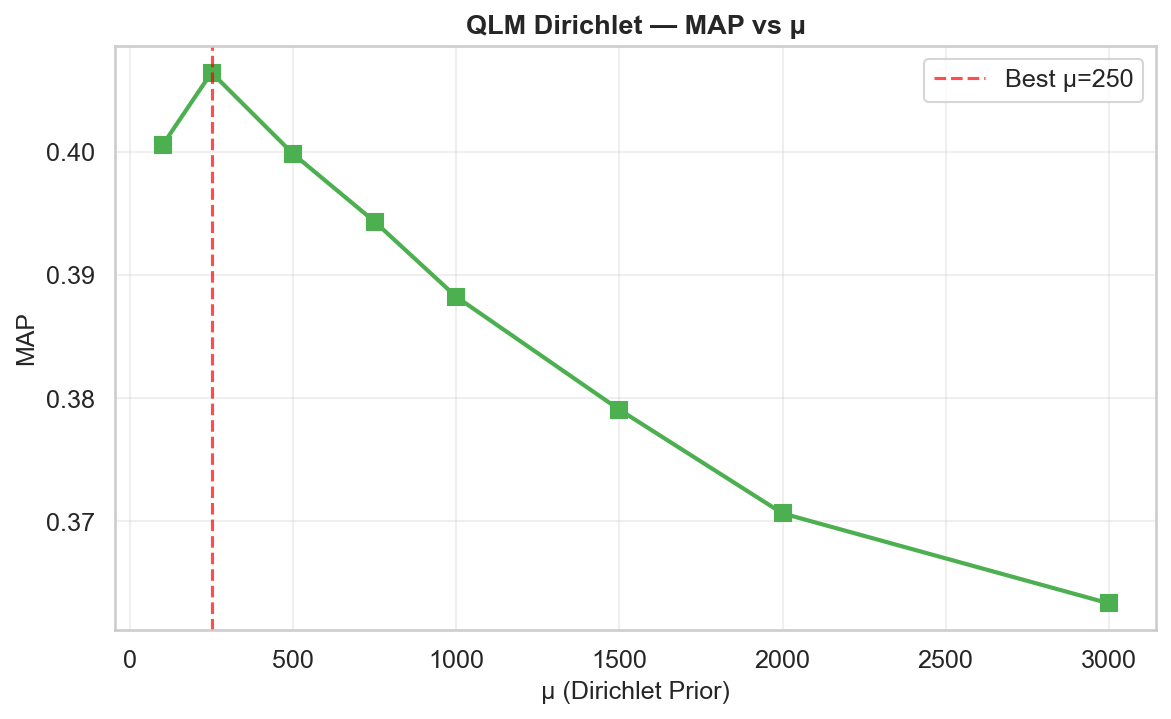
\includegraphics[width=0.6\textwidth]{figures/qlm_dirichlet_mu.png}
\caption{QLM Dirichlet --- MAP theo $\mu$.}
\label{fig:qlm_dir}
\end{figure}

% ---------------------------------------------------------------------------
\subsection{So sánh sau tinh chỉnh}
% ---------------------------------------------------------------------------

Biểu đồ so sánh hiệu suất các mô hình sau tinh chỉnh siêu tham số ở Hình~\ref{fig:comparison} cho thấy cái nhìn toàn diện về năm chỉ số đánh giá của bốn thuật toán xếp hạng tại ngưỡng cắt K bằng mười. Dựa vào biểu đồ, mô hình xác suất BM25 thể hiện sự áp đảo rõ rệt khi dẫn đầu ở các chỉ số Precision, Recall và F1-score. Mô hình TF-IDF cho thấy sự bền bỉ đáng kể khi duy trì hiệu suất bám đuổi sát nút với mô hình BM25 ở các mức độ đánh giá khác nhau. Hai biến thể của mô hình ngôn ngữ QLM Jelinek-Mercer và Dirichlet Prior có sự tương đồng rất cao về mặt phân bố điểm số và cùng xếp ở nhóm sau, phản ánh tính chất tương đương trong cơ chế làm trơn xác suất đối với tập văn bản ngắn. Điểm số MRR của tất cả các mô hình đều đạt mức rất cao (trên 0.80), cho thấy hệ thống luôn đưa được ít nhất một tài liệu liên quan lên vị trí cực kỳ cao (thường là vị trí thứ nhất hoặc thứ hai) trong danh sách trả về, đảm bảo trải nghiệm tốt cho người dùng cuối.

\begin{figure}[H]
\centering
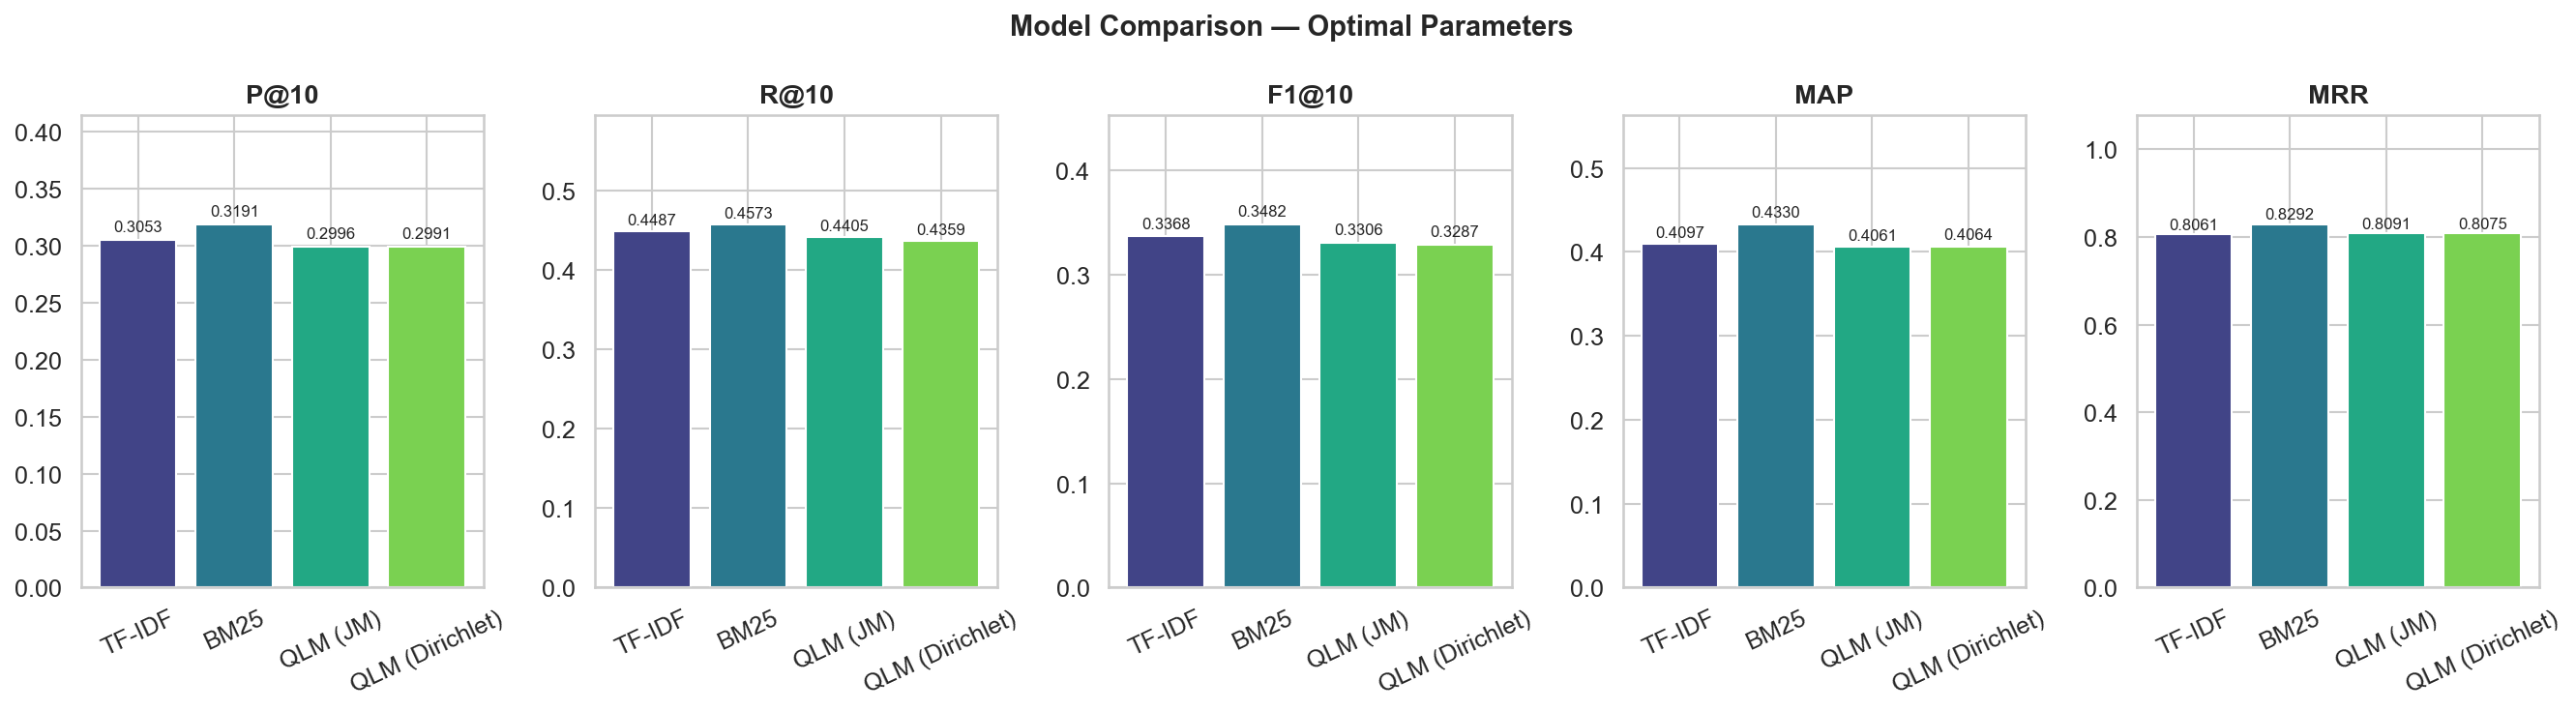
\includegraphics[width=0.85\textwidth]{figures/model_comparison_optimal.png}
\caption{So sánh hiệu suất các mô hình với tham số tối ưu.}
\label{fig:comparison}
\end{figure}

% ===========================================================================
\section{Tolerant Retrieval}
% ===========================================================================

Thực nghiệm đánh giá hiệu quả của module tìm kiếm chịu lỗi và sửa lỗi chính tả được tiến hành bằng cách lựa chọn mười câu truy vấn ngẫu nhiên và cố ý thay đổi ký tự để tạo ra các lỗi chính tả phổ biến như thay thế ký tự, thiếu ký tự hoặc gõ sai vị trí phím. Các câu truy vấn bị lỗi chính tả này được đưa vào kiểm thử trên hệ thống dưới hai điều kiện khác nhau là tắt tính năng sửa lỗi để tìm kiếm trực tiếp và bật tính năng tự động sửa lỗi dựa trên chỉ mục K-gram kết hợp khoảng cách Levenshtein. Kết quả hiệu suất được đối sánh trực tiếp với kết quả chạy câu truy vấn gốc ban đầu làm mốc so sánh tiêu chuẩn.

Hình~\ref{fig:tolerant} biểu diễn sự biến động hiệu suất tổng quan của hệ thống dưới ba trạng thái của câu truy vấn. Khi người dùng nhập câu truy vấn bị sai chính tả và hệ thống tắt tính năng sửa lỗi, điểm số MAP trung bình giảm mạnh từ 0.3277 xuống còn 0.2704, tương đương mức giảm khoảng mười bảy phần trăm, trong khi điểm số MRR cũng sụt giảm từ 0.7125 xuống còn 0.6322. Sự sụt giảm nghiêm trọng này xảy ra do các từ bị viết sai chính tả không thể tìm thấy các tài liệu chứa chúng trong chỉ mục ngược, dẫn đến việc mất mát các tài liệu liên quan quan trọng. Tuy nhiên, sau khi kích hoạt tính năng tự động sửa lỗi, điểm số MAP của hệ thống được khôi phục mạnh mẽ lên mức 0.3265, đạt hơn chín mươi chín phần trăm hiệu suất so với câu truy vấn gốc ban đầu, đồng thời điểm số MRR cũng quay trở lại mức 0.7125. Kết quả này chứng minh tính hiệu quả vượt trội và sự cần thiết của module sửa lỗi chính tả trong việc duy trì độ ổn định của hệ thống tìm kiếm trước các sai sót ngẫu nhiên của người dùng.

\begin{figure}[H]
\centering
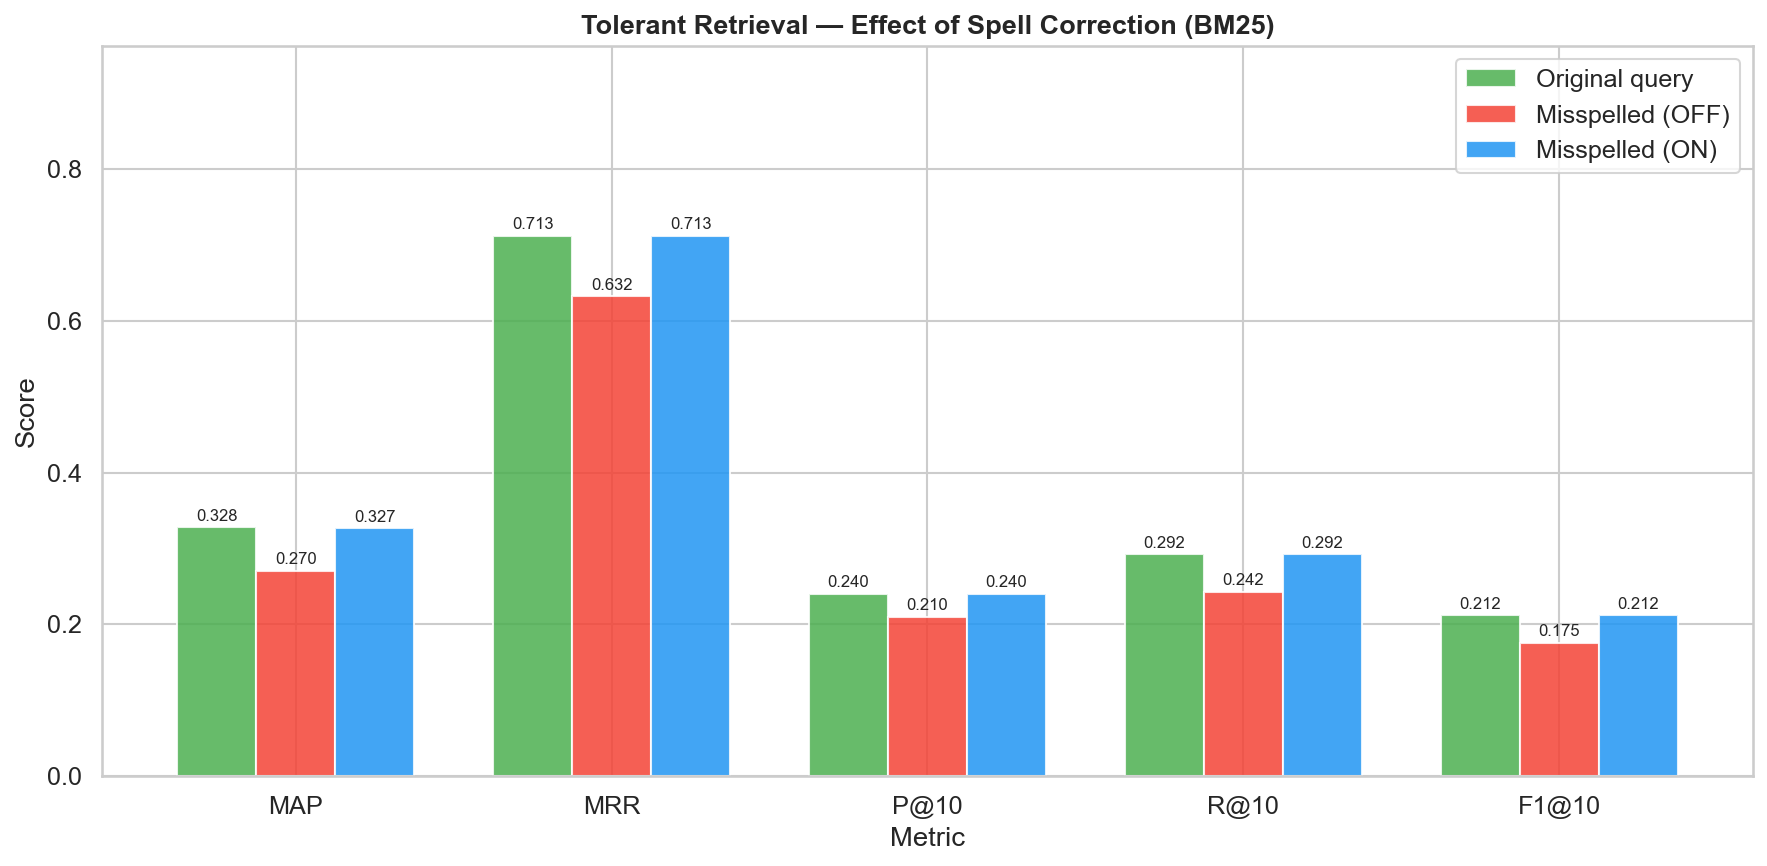
\includegraphics[width=0.75\textwidth]{figures/tolerant_comparison.png}
\caption{So sánh hiệu suất: truy vấn gốc, sai (không sửa), sai (có sửa).}
\label{fig:tolerant}
\end{figure}

Hình~\ref{fig:tolerant_pq} cung cấp cái nhìn chi tiết hơn về giá trị Average Precision của từng câu truy vấn trong số mười câu truy vấn thử nghiệm dưới ba điều kiện. Qua phân tích chi tiết, hầu hết các câu truy vấn sau khi sửa lỗi chính tả đều đạt được mức điểm số trùng khớp hoàn toàn với đường đồ thị của câu truy vấn gốc. Điều này phản ánh các lỗi sai tiêu biểu như viết thiếu chữ hoặc đảo ký tự đã được thuật toán sửa lỗi chuyển đổi chính xác về từ gốc chuẩn trong từ điển. Một số ít câu truy vấn có sự lệch điểm số rất nhỏ so với nguyên bản do từ được sửa đổi tuy có khoảng cách Levenshtein nhỏ nhất nhưng chưa phản ánh đúng hoàn toàn ngữ cảnh chuyên môn, tuy nhiên mức độ ảnh hưởng là không đáng kể và xu hướng chung vẫn là sự phục hồi hiệu suất tối đa.

\begin{figure}[H]
\centering
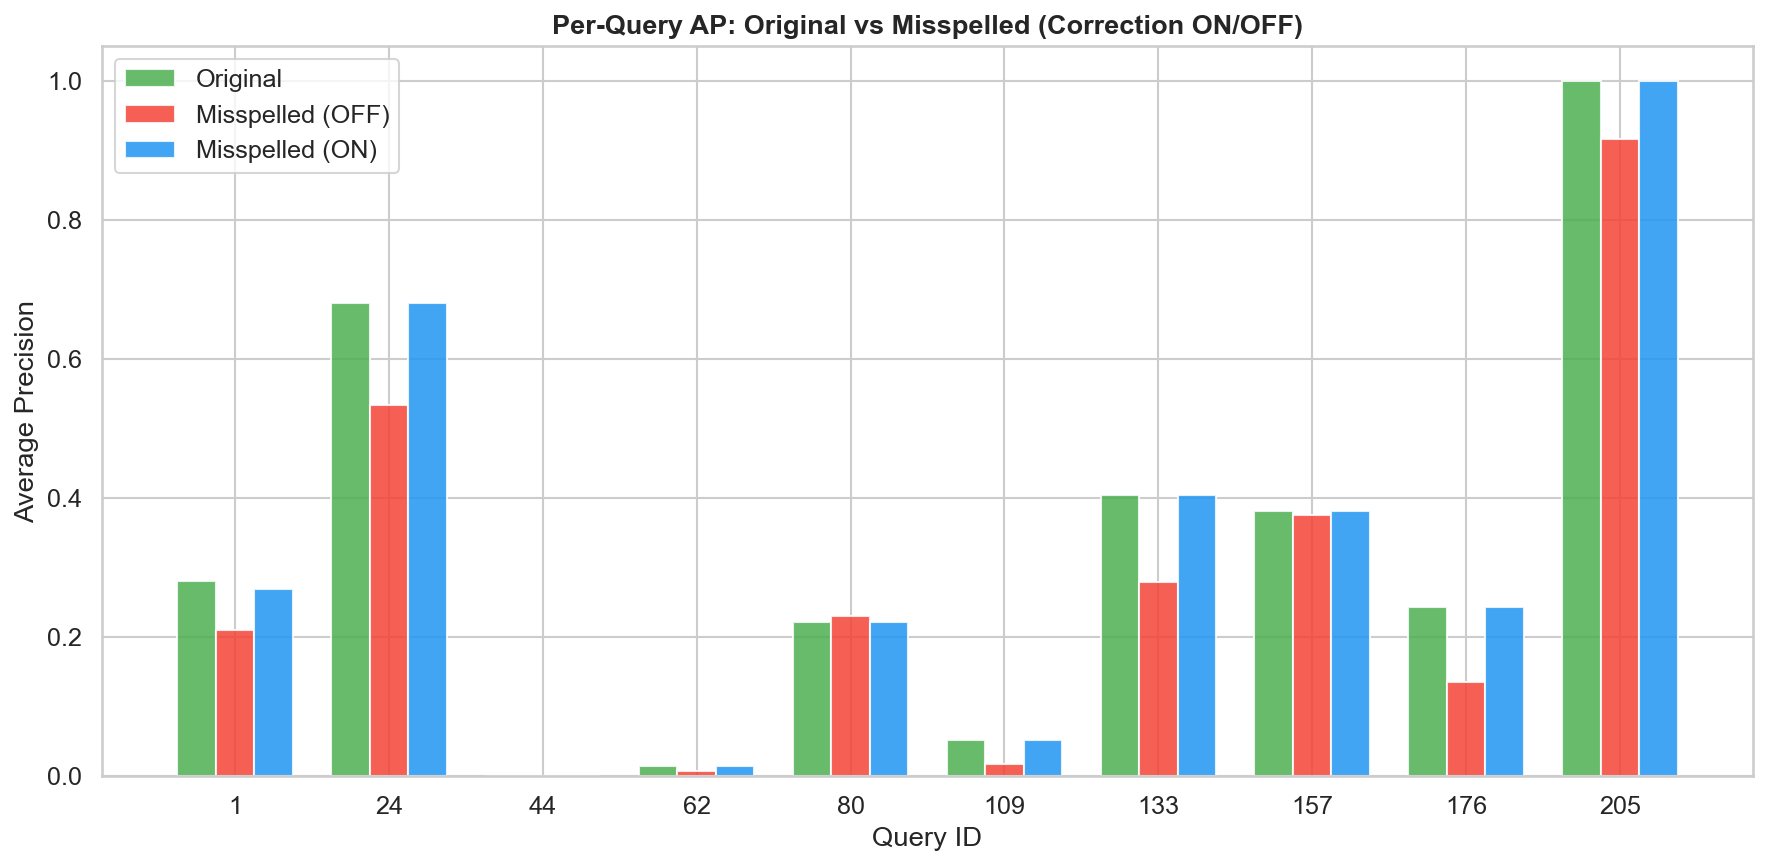
\includegraphics[width=0.85\textwidth]{figures/tolerant_per_query.png}
\caption{Average Precision theo từng truy vấn.}
\label{fig:tolerant_pq}
\end{figure}

% ===========================================================================
\section{Kết luận}
% ===========================================================================

Báo cáo đã trình bày quá trình xây dựng, đánh giá, và tinh chỉnh một hệ thống tìm kiếm thông tin trên bộ dữ liệu Cranfield. Bốn mô hình xếp hạng được cài đặt và so sánh, trong đó các mô hình xác suất (BM25 và QLM) thể hiện hiệu suất cao hơn so với TF-IDF cơ bản. Quá trình tinh chỉnh siêu tham số bằng Grid Search giúp tìm ra cấu hình phù hợp nhất cho từng mô hình. Module sửa lỗi chính tả dựa trên K-gram index và khoảng cách Levenshtein cho thấy khả năng phục hồi hiệu suất khi truy vấn bị viết sai. Tất cả các thành phần được tích hợp vào giao diện Streamlit, tạo thành hệ thống tìm kiếm hoàn chỉnh và dễ sử dụng.

\newpage

\section{Nhiệm vụ các thành viên}


\begin{center}
    {\textbf{Nhiệm vụ, vai trò các thành viên}}
\end{center}


\begin{longtable}{|>{\centering\arraybackslash}p{3cm}|
                      >{\centering\arraybackslash}p{4cm}|
                      p{7.5cm}|}
\hline
\textbf{Mã sinh viên} & \textbf{Họ và tên} & \textbf{Nhiệm vụ và vai trò} \\
\hline
\endfirsthead

\hline
\textbf{Mã sinh viên} & \textbf{Họ và tên} & \textbf{Nhiệm vụ, vai trò} \\
\hline
\endhead

B22DCKH004 & Ngô Việt Anh & Xây dựng cấu trúc chỉ mục ngược, chỉ mục K-gram, mô hình xếp hạng không gian vector TF-IDF, module đề xuất và sửa lỗi chính tả sử dụng khoảng cách Levenshtein (Edit Distance). \\
\hline
B22DCKH108 & Nguyễn Đình Tiến & Cài đặt mô hình xác suất Okapi BM25, mô hình Query Likelihood (QLM với Jelinek-Mercer smoothing và Dirichlet Prior smoothing), các hàm đánh giá hiệu suất (P@K, R@K, F1@K, MAP, MRR). \\
\hline
\end{longtable}

\end{document}
